\subsection{Overall Framework}
\label{sec:overall_framework}

HS-AeroTS implements the tasks defined in Section~\ref{sec:problem_formulation} and produces two related outputs: a runtime anomaly or normal decision with a conditional fault-domain prediction, and a traceable set of telemetry- and architecture-aware diagnostic evidence. As shown in Figure~\ref{fig:methodological_pipeline}, the method first aligns heterogeneous uORB-derived channels, constructs flight-aware windows, and converts each window into temporal-statistical features. Stage 1 performs binary runtime anomaly detection, and Stage 2 performs four-class fault-domain diagnosis for anomalous windows. For a Stage 2 prediction, TreeSHAP contributions are aggregated from statistical features to telemetry channels, PX4 uORB topics, and functional subsystems. For firmware-matching data, topic evidence is then propagated through a commit-specific static uORB graph to produce software-module suspects for engineering inspection. The data-processing, diagnosis, explanation, and architecture-aware layers are described below in this order; each layer has its own input, output, and evaluation boundary.

\begin{figure}[!t]
    \centering
    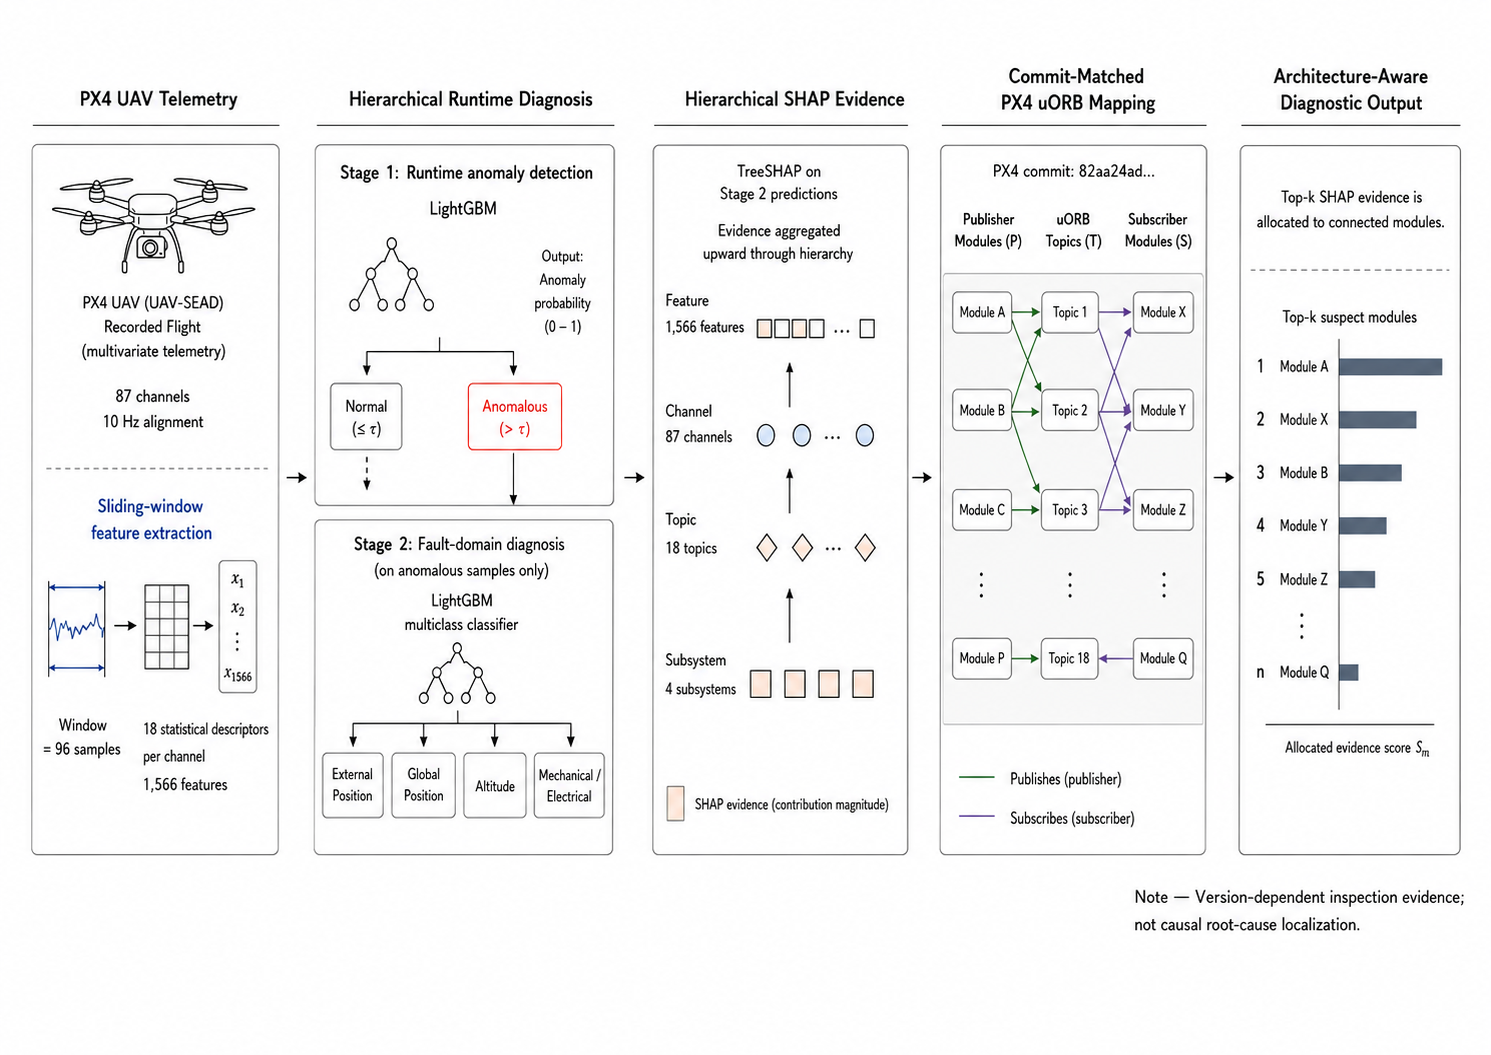
\includegraphics[width=\textwidth]{figures/figure-2-hs-aerots-fl-methodological-pipeline-preview2.png}
    \caption{Methodological pipeline. Runtime telemetry is transformed into temporal-statistical windows for anomaly detection and conditional fault-domain diagnosis. TreeSHAP evidence is aggregated through the feature--channel--topic--subsystem hierarchy, while a static source-tree graph reconstructed at the majority PX4 firmware commit maps topic evidence to software-module inspection candidates. Ground-truth-anomaly-conditioned and Stage-1-gated evaluations are reported separately. The architecture branch is associative and version-dependent, not causal or deployment-build validated.}
    \label{fig:methodological_pipeline}
\end{figure}
